\section{Лекция 2. Метод Ньютона. Two-slope тест}
\subsection{Введение}
{\bf Опр.1.16}
Функция $q:\mathbb{R}^n \to \mathbb{R}$ называется {\bf квадратичной}, если матрица $Q \in \mathbb{R}^{[n]\times[n]}$ симметричная и при $c \in \mathbb{R}^n$, $\gamma \in \mathbb{R}$ выполняется для всех $x \in \mathbb{R}^n$:
\begin{center} $q(x)=x^TQx+<c,x>+\gamma$ \end{center}

{\bf Опр.1.17}
Матрица $Q \in \mathbb{R}^{[n]\times[n]}$ {\bf положительно определена, положительно полуопределена, отрицательно определена, отрицательно полуопределена}, когда для всех $x \in \mathbb{R}^n \setminus \mathbb{O}_n$ соответственно:\\
$x^TQx>0,\\ x^TQx \ge 0,\\ x^TQx<0,\\ x^TQx \le 0$.\\ Матрица не определена, когда она ни положительно, ни отрицательно полуопределена.\\

{\bf Теорема 1.18}
Симметрическая матрица $Q \in \mathbb{R}^{[n]\times[n]}$ положительно определена, положительно полуопределена, отрицательно определена, отрицательно полуопределена, когда все собственные значения $Q$ положительны, не отрицательны, отрицательны, не положительны. Матрица не определена, когда она содержит и положительные, и отрицательные собственные значения.\\

{\bf Теорема 1.19}
Пусть функция $q(x):\mathbb{R}^n \to \mathbb{R}$ --- квадратичная и  $q(x)=x^TQx+<c,x>+\gamma \text{, } q(x)$ (строго) выпукла вниз/вверх, когда для всех
 $x \in \mathbb{R}^n$ матрица $Q$ положительно/отрицательно полуопределена (определена).\\

{\bf Теорема 1.20}
Дважды непрерывно дифференцируемая функция\\ $f:\mathbb{R}^n \to \mathbb{R}$ выпукла вниз/вверх, когда для всех $x \in \mathbb{R}^n$ матрица Гессе положительно/отрицательно полуопределена. Если при этом матрица Гессе всюду положительно/отрицательно определена, то $f$ строго выпукла вниз/вверх.\\

{\bf Замечание 1.21} \\ Для квадратичной функции $q(x)=x^TQx+<c,x>+\gamma$ характер выпуклости полностью определяется частью с квадратами, так как для любого $x^*:$
\begin{center}1. $grad_{x^*}q=2Qx^*+c$\\ 2. $hess_{x^*}q=2Q$ \end{center}









\subsection{Необходимый критерий}
{\bf Теорема 1.22 (необходимый критерий)}
Если функция\\ $f:\mathbb{R}^n \supseteq X \to \mathbb{R}$ принимает локальный экстремум во внутренней точке $x^* \in int(X)$, в которой $f$ дифференцируема, то $grad_{x^*}f=\mathbb{O}_n$.\\

{\bf Опр.1.23}
Для каждой дифференцируемой функции $f:\mathbb{R}^n \supseteq X \to \mathbb{R}$ ($X$ открыто) точка $x^* \in X$, для которой $grad_{x^*}f=\mathbb{O}_n$, называется {\bf стационарной точкой}.\\

{\bf Следствие 1.24}
Стационарные точки --- единственные кандидаты на локальный экстремум дифференцируемой функции (для открытых множеств).\\

\subsection{Достаточный критерий второго порядка}
{\bf Теорема 1.25 (достаточный критерий второго порядка)}
Пусть $f:\mathbb{R}^n \supseteq X \to \mathbb{R}$ ($X$ открыто) дважды непрерывно дифференцируема на $X$ и пусть $x^* \in X$ --- стационарная точка $f$. Тогда:
\begin{enumerate}
\item Если $hess_{x^*}f$ положительно определена, то $f$ принимает в $x^*$ локальный минимум;
\item Если $hess_{x^*}f$ отрицательно определена, то $f$ принимает в $x^*$ локальный максимум;
\item Если $hess_{x^*}f$ не определена, то в $x^*$ нет локального экстремума.
\end{enumerate}

\subsection{ Идея метода Ньютона}
\begin{itemize}
\item Пусть $f:\mathbb{R}^n \to \mathbb{R}$ дважды непрерывно дифференцируема на $\mathbb{R}^n$ и:
   \begin{itemize}
   \item $hess_xf$ положительно определена для всех $x \in \mathbb{R}^n$
   \item $f$ имеет глобальный минимум, который также достигается в единственной    стационарной точке $x^{min} \in \mathbb{R}^n$
   \end{itemize}
\item Стратегия: генерируем последовательность $x^{(0)}, x^{(1)}, \dots \in \mathbb{R}^n$, причем $\lim_{k \to \infty} x^{(k)}=x^{min}$
\item Для всех $k$:
   \begin{itemize}
   \item выбираем необходимое направление $d^{(k)} \in \mathbb{R}^n$
   \item определяем $ x^{(k+1)}$ как (приблизительное) оптимальное решение одномерной проблемы минимума $min \{f(x^{(k)}+td^{(k)}) \mid t \in \mathbb{R} \}$.
   \end{itemize}
\end{itemize}

{\bf Определение направления $d^{(k)}$}\\
\checkmark Квадратичная функция\\
$q^{(k)}(x):=\frac{1}{2} (x-x^{(k)})^T(hess_{x^{(k)}}f)(x-x^{(k)})+<grad_{x^{(k)}}f,x-x^{(k)}>
+f(x^{(k)})=\\=x^TQ^{(k)}x+<c^{(k)}, x>+\gamma^{(k)}$\\
где\\
$Q^{(k)}=\frac{1}{2} hess_{x^{(k)}}f\\
c^{(k)}=grad_{x^{(k)}}f-(hess_{x^{(k)}}f)x^{(k)}\\
\gamma^{(k)}=f(x^{(k)})+\frac{1}{2} x^{(k)^T}(hess_{x^{(k)}}f)x^{(k)}$\\
хорошо приближает функцию $f$ в окрестности $x^{(k)}$.\\
\checkmark функция $q^{(k)}$ строго выпукла с единственной точкой минимума $\tilde{x}$/\\

\checkmark $d^{(k)}=\tilde{x}-x^{(k)}$\\

\checkmark $\mathbb{O}_n=grad_{\tilde{x}}q=2Q^{(k)} \tilde{x}+c^{(k)}$\\

\checkmark $Q^{(k)}$ положительно определена и обратима, то после подстановки получаем:\\

$\tilde{x}=x^{(k)}-(hess_{x^{(k)}}f)^{-1}grad_{x^{(k)}}f$
значит $d^{(k)}=-(hess_{x^{(k)}}f)^{-1}grad_{x^{(k)}}f$\\

\subsection{ Минимизация с использованием Two-Slope-Test }
\checkmark Пусть $x^{(k)}$ не стационарная точка $f$.\\

\checkmark Пусть $\phi_{k}:\mathbb{R}^n \to \mathbb{R}$ такая, что $\phi_{k}(t)=f(x^{(k)}+td^{(k)})$.\\

\checkmark $d^{(k)}$ - направление спуска, значит $\phi^{'}_{k}(0)<0$.\\

\checkmark Идеальный случай: $x^{(k+1)}=x^{(k)}+\tau^{*}_{k}d^{(k)}$ для аргумента минимизации $\tau^{*}_{k}$ задачи $\min( \phi_{k}(t)|t\in\mathbb{R})$\\
\checkmark Вместо этого: выберем исходные параметры $1>\alpha_{1}>\frac{1}{2}>\alpha_{0}>0$ а затем найдем такой $x^{(k+1)}=x^{(k)}+\tau_{k}$ для $\tau_{k}>0$ такого, что условия Two-Slope выполняются\\
\begin{center}$\phi_{k}(0)+\alpha_{1}\phi^{'}_{k}(0)\tau\leq\phi_{k}(\tau)\leq\phi_{k}(0)+\alpha_{2}\phi^{'}_{k}(0)\tau$\end{center}

\checkmark Определяем при помощи проверки такую $u=1,2,4,8,...$, что $\phi_{k}(0)+\alpha_{1}\phi^{'}_{k}(0)u\leq\phi_{k}(u)$\\
\checkmark В случае $\phi_{k}(u)\leq\phi_{k}(0)+\alpha_{2}\phi^{'}_{k}(0)u: \tau_{k}=u$\\

\checkmark В противном случае $l=0$ и делаем тоже самое для $\phi_{k}(l)\leq\phi_{k}(0)+\alpha_{2}\phi^{'}_{k}(0)l$\\
\checkmark Проверяем оба неравенства из условий Two-Slope для $\tau=\frac{u-l}{2}$. Если выполняются оба, то $\tau_{k}=\tau$\\
Если не выполняется первое, то $l=\tau$ и снова проверяем условия для пересчитанного $\tau$\\
Если не выполняется второе, то $u=\tau$ и снова проверяем условия для пересчитанного $\tau$\\
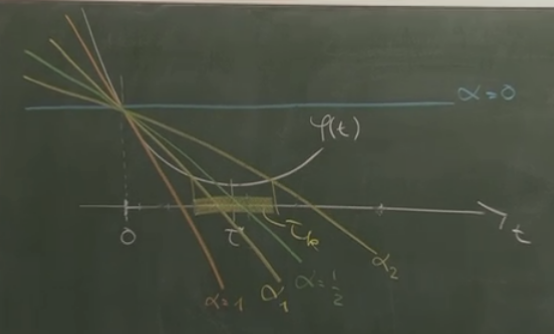
\includegraphics[scale=0.8]{image1.png}


{\bf Замечание} Метод находит нужное $\tau$ за конечное число шагов
\newpage
\subsection{Анализ метода Ньютона}

{\bf Предложение 1.26} Пусть $f: \mathbb{R}^n \to \mathbb{R}$ дважды непрерывно дифференцируемая на $\mathbb{R}^n$ со всюду положительно определенной матрице Гессе и $x^{(0)}\in\mathbb{R}^n$ такое, что множество $X^{0}:=\{x\in\mathbb{R}^{n}| f(x)\leq f(x^{(0)})\}$ ограничено, то сходится последовательность, генерируемая методом Ньютона и тестом Two-Slope к точке, в которой $f$ достигает своего минимума.\\

{\bf Замечание} Для всех достаточно больших k выполняется условие:
\begin{center}$\|x^{(k+1)}-x^{min}\|\leq \frac{L}{2m}\|x^{(k)}-x^{min}\|^{2}$\end{center}
где L - константа Липшица для функции $x\rightarrow hess_{x}f$ и m - наименьшее собственное значение $ hess_{x}f$ на $X^{0}$. В частности, при хорошем выборе начальной точки получается квадратичная сходимость.

{\Large \bf Лекция 2: выпуклые множества и конусы}\\

\subsection{Выпуклые множества}

{\bf Опр.2.1}
Множество $X \subseteq \mathbb{R}^n$ называется {\bf выпуклым} в случае, если для любых $x,y \in X$: $\lambda x+(1-\lambda)y \in X$ для всех $0 \le \lambda \le 1$.\\

Множество выпуклое, если оно с любыми двумя своими точками содержит отрезок их соединяющий.\\
\begin{center}
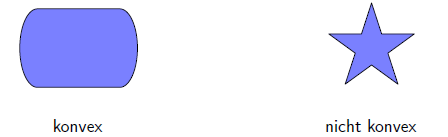
\includegraphics[scale=0.8]{image2.png}
\end{center}
{\bf Выпуклые функции над выпуклыми множествами}

{\bf Опр.2.2}
Пусть $X \subseteq \mathbb{R}^n$ выпукло. Функция $f:X \to \mathbb{R}$ называется выпуклой вниз(вверх), если для всех $x,y \in X$, $0 \le \lambda \le 1$:
\begin{center}
$f(\lambda x+(1-\lambda )y) \leq\left(\geq\right)  \lambda f(x)+(1-\lambda)f(y)$
\end{center}

{\bf Замечание 2.3}
Если выпуклая вниз/вверх функция на выпуклом множестве принимает в точке локальный минимум/максимум, то она там также принимает глобальный минимум/максимум.\\

{\bf Наблюдение 2.4} Пусть функция $f:\mathbb{R}^n \to \mathbb{R}$ выпуклая, то для каждого $\alpha\in\mathbb{R}$ множество $\{x\in\mathbb{R}^n: f(x)\leq a\}$ выпукло.\\
\begin{center}
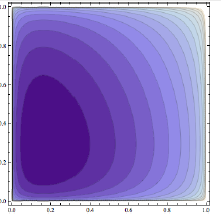
\includegraphics[scale=0.8]{image3.png}
\end{center}

{\bf Эллипсоиды}

{\bf Замечание 2.5} Для положительно определенной симметричной матрицы $Q\in\mathbb{R}^{n\times n}$ и $z\in\mathbb{R}^n$  определяется выпуклый и компактный эллипсоид с центром в z: \\
\begin{center}
$Ell(z,Q):=\{x\in\mathbb{R}^n|(x-z)^T Q^{-1} (x-z)\leq 1\}$
\end{center}

Самым простым эллипсоидом является шар. Это эллипсоид с единичной матрицей. Полуоси эллипсоида равны корням из соответствующих собственных значений матрицы.
\begin{center}
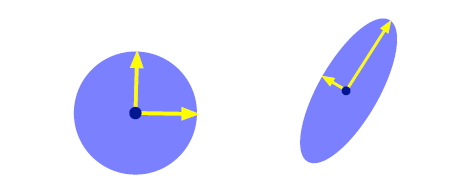
\includegraphics[scale=0.8]{image4.png}
\end{center}
{\bf Наблюдение 2.6}
Пусть $I$ --- множество индексов (любой мощности) и $X_i \subseteq \mathbb{R}^n$ --- выпуклое множество $(i \in I)$. Тогда $\bigcap_{i \in I}X_i$ также выпукло.\\

\subsection{Оболочки}
{\bf Выпуклые оболочки}

{\bf Опр.2.7}
Для $X \subseteq \mathbb{R}^n$ будем называть
\begin{center}
$conv X:=\bigcap$ $\{X^* \subseteq \mathbb{R}^n \mid X \subseteq X^*, X^* $ выпукло\}
\end{center}
{\bf выпуклой оболочкой} $X$.\\

{\bf Линейная оболочка:}
\begin{center}
$lin X:=\bigcap \{L \subseteq \mathbb{R}^n \mid X \subseteq L, L $ линейное подпространство\}
\end{center}

{\bf Аффинная оболочка:}
\begin{center}
$aff X:=\bigcap \{A \subseteq \mathbb{R}^n \mid X \subseteq A, A $ аффинное подпространство\}
\end{center}

\vspace{8pt}
Для $x^{(1)}, \dots , x^{(r)} \in \mathbb{R}^n$ и $\lambda_1, \dots , \lambda_r \in \mathbb{R}$
\begin{center}
$\sum_{i=1}^r \lambda_ix^{(i)}$
\end{center}
{\bf линейная комбинация} $x^{(1)}, \dots , x^{(r)}$.

\begin{itemize}
\item В случае $\sum_{i=1}^r \lambda_i=1$: {\bf аффинная комбинация}
\item В случае $\lambda_1, \dots , \lambda_r \ge 0$: {\bf коническая комбинация}
\item Конические аффинные комбинации: {\bf выпуклые комбинации}
\end{itemize}

{\bf Замечание 2.8}
Выпуклая / линейная / аффинная оболочка $X \subseteq \mathbb{R}^n$ --- это множество всех выпуклых / линейных / аффинных комбинаций (конечного числа) точек из $X$.\\ 